%%%%%%%%%%%%%%%%%%%%%%%%%%%%%%%%%%%%%%%%%%%%%%%%%%%%%%%%%%%%%%%%%%%%%%%%%%%%%%%%%%%%%%%%%%%%%%%%%%%%%%%%%%%%%%%%%%%%%%%%%%%%%%%%%%%%%%%%%%%%%%%%%%%%%%%%%%%%%%%%%%%%%%%%%%%%%%%%%%%%%%%%%%%%
% Written By Michael Brodskiy
% Class: Thermodynamics & Statistical Mechanics
% Professor: A. Stepanyants
%%%%%%%%%%%%%%%%%%%%%%%%%%%%%%%%%%%%%%%%%%%%%%%%%%%%%%%%%%%%%%%%%%%%%%%%%%%%%%%%%%%%%%%%%%%%%%%%%%%%%%%%%%%%%%%%%%%%%%%%%%%%%%%%%%%%%%%%%%%%%%%%%%%%%%%%%%%%%%%%%%%%%%%%%%%%%%%%%%%%%%%%%%%%

\documentclass[12pt]{article} 
\usepackage{alphalph}
\usepackage{tipa}
\usepackage[utf8]{inputenc}
\usepackage[russian,english]{babel}
\usepackage{titling}
\usepackage{amsmath}
\usepackage{graphicx}
\usepackage{enumitem}
\usepackage{amssymb}
\usepackage[super]{nth}
\usepackage{everysel}
\usepackage{ragged2e}
\usepackage{geometry}
\usepackage{multicol}
\usepackage{fancyhdr}
\usepackage{cancel}
\usepackage{siunitx}
\usepackage{physics}
\usepackage{tikz}
\usepackage{mathdots}
\usepackage{yhmath}
\usepackage{cancel}
\usepackage{color}
\usepackage{array}
\usepackage{multirow}
\usepackage{gensymb}
\usepackage{tabularx}
\usepackage{extarrows}
\usepackage{booktabs}
\
\usepackage{mhchem}
\geometry{top=1.0in,bottom=1.0in,left=1.0in,right=1.0in}
\newcommand{\subtitle}[1]{%
  \posttitle{%
    \par\end{center}
    \begin{center}\large#1\end{center}
    \vskip0.5em}%

}
\usepackage{hyperref}
\hypersetup{
colorlinks=true,
linkcolor=blue,
filecolor=magenta,      
urlcolor=blue,
citecolor=blue,
}

\urlstyle{same}
\usepackage{fancyhdr}
\pagestyle{fancy}
\lhead[\textsc{Fall 2023}]{\textsc{Fall 2023}}
\chead[\textit{Thermodynamics Final Equation Sheet}]{\textit{Thermodynamics Final Equation Sheet}}
\rhead[\textsc{Phys-4305}]{\textsc{Phys-4305}}
\cfoot[\thepage]{\thepage}

\pagenumbering{gobble}
\begin{document}


\begin{multicols}{2}

  \begin{equation*}
    g(N,s)=\frac{N!}{\left(\frac{1}{2}N+s\right)\left( \frac{1}{2}N-s \right)}=\frac{N!}{N_{\uparrow}!N_{\downarrow}!}
  \end{equation*}

  \begin{equation*}
    g(N,s)\approx \sqrt{\frac{2}{\pi N}}2^Ne^{-\frac{2s^2}{N}}
  \end{equation*}

\end{multicols}

\vspace{-20pt}

\begin{multicols}{2}

  \begin{equation*}
    U(s)=-2smB
  \end{equation*}
    
  \begin{equation*}
    2s=N_{\uparrow}-N_{\downarrow}
  \end{equation*}

\end{multicols}

\vspace{-30pt}

\begin{multicols}{2}

  \begin{equation*}
    \begin{split}
    \sigma(N,s)&=\ln(g(N,s))\\
    S&=k_B\sigma
    \end{split}
  \end{equation*}
    
  \begin{equation*}
    \begin{split}
      \frac{1}{\tau}&=\left( \frac{\partial \sigma}{\partial U} \right)_{N,V}\\
      \tau&=k_BT
    \end{split}
  \end{equation*}

\end{multicols}

\vspace{-30pt}

\begin{multicols}{2}

  \begin{equation*}
    \begin{split}
      \text{\underline{Accessible States} } (s=s_1+s_2):\\
      g(s)=\sum_s g_1(s_1)g_2(s-s_1)
    \end{split}
  \end{equation*}
    
  \begin{equation*}
    \begin{split}
      \text{System/Reservoir State Probability:}\\
      P(\varepsilon_s)=\frac{1}{z}e^{-\frac{\varepsilon_s}{\tau}}
    \end{split}
  \end{equation*}

\end{multicols}

\vspace{-30pt}

\begin{multicols}{2}

  \begin{equation*}
    z=\sum_s e^{-\frac{\varepsilon_s}{\tau}}
  \end{equation*}
    
  \begin{equation*}
    P=-\left( \frac{\partial U}{\partial V} \right)_\sigma=\tau\left( \frac{\partial\sigma}{\partial V} \right)_U=-\left( \frac{\partial F}{\partial V} \right)_\tau
  \end{equation*}

\end{multicols}

\vspace{-30pt}

\begin{multicols}{2}

  \begin{equation*}
    F=U-\tau\sigma\quad\text{min. in eq. with const } \tau,V
  \end{equation*}

  \begin{equation*}
    F=-\tau\ln(z)\quad\text{ to derive }P,\sigma
  \end{equation*}

\end{multicols}

\vspace{5pt}

\hline

\begin{center}
  \underline{Ideal Monatomic Gas}
\end{center}

\vspace{-40pt}

\begin{multicols}{2}

  \begin{equation*}
    \text{Given $N$ atoms: }z_N=\frac{(n_QV)^N}{N!}
  \end{equation*}

  \begin{equation*}
    \text{If }n=\frac{N}{V}<<n_Q,\quad n_Q=\left(\frac{M\tau}{2\pi\hbar^2}\right)^{\frac{3}{2}}
  \end{equation*}

\end{multicols}

\vspace{-25pt}

\begin{multicols}{3}

  \begin{equation*}
    PV=N\tau
  \end{equation*}

  \begin{equation*}
    \sigma=N\left[ \ln\left( \frac{n_Q}{n} \right)+\frac{5}{2} \right]
  \end{equation*}

  \begin{equation*}
    C_V=\frac{3}{2}N
  \end{equation*}

\end{multicols}

\hline

\vspace{5pt}

\begin{flushleft}
A process is reversible if the system remains infinitesimally close to the equilibrium state at all times during the process.
\end{flushleft}

\vspace{-30pt}

\begin{multicols}{2}

  \begin{equation*}
    \text{Average in Mode at freq. $\omega$: }\langle s\rangle=\frac{1}{e^{\frac{\hbar\omega}{\tau}}-1}
  \end{equation*}

  \begin{equation*}
    \text{Energy Density at $\tau$: }\langle s\rangle=\frac{U}{V}=\frac{\pi^2}{15\hbar^3c^3}\tau^4
  \end{equation*}

\end{multicols}

\vspace{-30pt}

\begin{multicols}{2}

  \begin{equation*}
    \text{Radiant energy per vol: }U_\omega=\frac{\hbar}{\pi^2c^3}\frac{\omega^3}{e^{\frac{\hbar\omega}{\tau}}-1}
  \end{equation*}

  \begin{equation*}
    \text{Flux Density: }J_U=\sigma_BT^4,\,\sigma_B=\frac{\pi^2k_B^4}{60\hbar^3c^2}
  \end{equation*}

\end{multicols}

\vspace{-20pt}

$$\text{Heat Capacity of Dielectric Solid: } C_V=\frac{12\pi^4Nk_B}{5}\left( \frac{T}{\theta} \right)^3\rightarrow\theta=\left( \frac{\hbar\omega}{k_B} \right)\left( \frac{6\pi^2N}{V} \right)^{\frac{1}{3}}$$

\begin{multicols}{2}

  \begin{equation*}
    \mu=\left( \frac{\partial F}{\partial N} \right)_{\tau,V}=\left( \frac{\partial U}{\partial N} \right)_{\sigma,V}=-\tau\left( \frac{\partial\sigma}{\partial N} \right)_{U,V}
  \end{equation*}

  \begin{equation*}
    \text{In diffusive equilibrium if: }\mu_1=\mu_2
  \end{equation*}

\end{multicols}

\begin{multicols}{2}

  \begin{equation*}
    \begin{split}
    \mu&=\mu_{int}+\mu_{ext}\\
    \mu_{int}&=\tau\ln\left( \frac{n}{n_Q} \right)\\
    \mu_{ext}&=\frac{U_{ext}}{N}
    \end{split}
  \end{equation*}

  \begin{equation*}
    \begin{split}
      \text{Gibbs Factor: }P(N,\varepsilon_s)=\frac{e^{\frac{N\mu-\varepsilon_s}{\tau}}}{\text{\textrevepsilon}}\\
      \text{Prob. chem. potential $\mu$ and temp $\tau$}\\
      \text{has $N$ particles in q.s. $s$ of energy $\varepsilon_s$}
    \end{split}
  \end{equation*}

\end{multicols}

\vspace{-20pt}

\begin{multicols}{2}

  \begin{equation*}
    \text{\textrevepsilon}=\sum_N\sum_{s} e^{\frac{N\mu-\varepsilon_s}{\tau}}
  \end{equation*}

  \begin{equation*}
    \lambda=e^{\frac{\mu}{\tau}}\rightarrow\text{\textrevepsilon}=\sum\lambda^Ne^{-\frac{\varepsilon_s}{\tau}}
  \end{equation*}

\end{multicols}

\begin{multicols}{2}

  \begin{equation*}
    \text{Therm. Average: }\langle N\rangle=\lambda\frac{\partial}{\partial \lambda}\ln(\text{\textrevepsilon})
  \end{equation*}

  \begin{equation*}
    \text{Quant. Particle in Box: }\varepsilon=\frac{\hbar^2\pi^2}{2mL^2}(n_x^2+n_y^2+n_z^2)
  \end{equation*}

\end{multicols}

\begin{multicols}{2}

  \begin{equation*}
    U=\tau^2\left( \frac{\partial\,\ln(z)}{\partial\tau} \right)_V
  \end{equation*}

  \begin{equation*}
    W=PA\Delta x=P\Delta V
  \end{equation*}

\end{multicols}

\begin{multicols}{2}

  \begin{equation*}
    \tau\,d\sigma=dU+P\,dV
  \end{equation*}

  \begin{equation*}
    \int_{-\infty}^\infty e^{-\alpha^2n^2}\,dn=\frac{\sqrt{\pi}}{2\alpha}
  \end{equation*}

\end{multicols}

\vspace{-30pt}

\begin{multicols}{2}

  \begin{equation*}
    \sigma=-\left( \frac{\partial F}{\partial \tau} \right)_{V,N}
  \end{equation*}

  \begin{equation*}
    \langle N\rangle=\sum_N\sum_sN\cdotP(N,\varepsilon_s)=\tau\left( \frac{\partial \ln(\text{\textrevepsilon})}{\partial\mu} \right)_{\tau,V}
  \end{equation*}

\end{multicols}

\begin{multicols}{2}

  \begin{equation*}
    \langle \varepsilon_s\rangle=\sum_N\sum_s\varepsilon_s\cdotP(N,\varepsilon_s)=\tau^2\left( \frac{\partial \ln(\text{\textrevepsilon})}{\partial\tau} \right)_{\mu,V}+\tau\mu\left( \frac{\partial\ln(\text{\textrevepsilon})}{\partial\mu} \right)_{\tau,V}
  \end{equation*}


  \begin{equation*}
  \hspace{60pt}
    f(\varepsilon_n) \text{ avg. occupancy}
  \end{equation*}

\end{multicols}

\vspace{-25pt}

\begin{multicols}{3}

  \begin{equation*}
    \begin{split}
    \text{\underline{Bose-Einstein:}}\\
    f(\varepsilon_n)=\frac{1}{e^{\frac{\varepsilon_n-\mu}{\tau}}-1}
    \end{split}
  \end{equation*}

  \begin{equation*}
    \begin{split}
    \text{\underline{Fermi-Dirac:}}\\
    f(\varepsilon_n)=\frac{1}{e^{\frac{\varepsilon_n-\mu}{\tau}}+1}
    \end{split}
  \end{equation*}

  \begin{equation*}
    \begin{split}
    \text{\underline{Classical Limit:}}\\
    f(\varepsilon_n)=e^{\frac{\mu-\varepsilon_n}{\tau}}
    \end{split}
  \end{equation*}

\end{multicols}

\vspace{10pt}

\begin{center}
\begin{tabular}[H]{|c|c|c|c|c|}
  \hline
  & $\Delta U$ & $\Delta\sigma$ & $W$ & $Q$\\
  \hline
Rev. Isothermal & 0 & $N\ln\left( \frac{V_2}{V_1} \right)$ & $-N\tau\ln\left( \frac{V_2}{V_1} \right) \right)$ & $N\tau\ln\left( \frac{V_2}{V_1} \right)$\\
  \hline
Rev. Isentropic  & $-\frac{3}{2}N\tau_1\left[ 1-\left( \frac{V_1}{V_2} \right)^{\frac{2}{3}} \right]$ & 0 & $-\frac{3}{2}N\tau_1\left[ 1-\left( \frac{V_1}{V_2} \right)^{\frac{2}{3}} \right]$ & 0\\
  \hline
  Irrev. Expansion  & 0 & $N\ln\left( \frac{V_2}{V_1} \right)$ & 0 & 0\\
  \hline
\end{tabular}
\end{center}

\noindent\fbox{%
    \parbox{\textwidth}{%

      \vspace{-10pt}

  \begin{center}
    \underline{Constants}
  \end{center}

  \vspace{-30pt}

  \begin{multicols}{3}

    \begin{equation*}
      k_B=1.381\cdot10^{-23}\left[ \frac{\si{\joule}}{\si{\kelvin}} \right]
    \end{equation*}

    \begin{equation*}
      \sigma_B=5.67\cdot10^{-8}\left[ \frac{\si{\joule}}{\si{\meter\squared\second\kelvin^4}} \right]
    \end{equation*}

    \begin{equation*}
      c=3\cdot10^8\left[ \frac{\si{\meter}}{\si{\second}} \right]
    \end{equation*}

  \end{multicols}

    }%
}

\begin{multicols}{2}

  \begin{equation*}
    \begin{split}
    \text{Energy of Highest-Filled Orbital}\\
    \text{\underline{of Fermi Gas (spin 1/2):}}\\
    \varepsilon_f=\frac{\hbar^2}{2M}\left( \frac{3\pi^2N}{V} \right)^{\frac{2}{3}}
    \end{split}
  \end{equation*}

  \begin{equation*}
    \begin{split}
    \text{\underline{Ground State Kinetic Energy:}}\\
    U_o=\frac{3}{5}N\varepsilon_f\\
    \text{\underline{Density of Orbitals:}}\\
    \mathcal{D}(\varepsilon_f)=3N/2\varepsilon_f
    \end{split}
  \end{equation*}

\end{multicols}

\vspace{-30pt}

\begin{multicols}{2}

  \begin{equation*}
    \begin{split}
      \text{\underline{Heat Capacity of Electron Gas ($\tau<<\tau_F$):}}\\
      C_{el}=\frac{1}{3}\pi^2\mathcal{D}(\varepsilon_f)\tau\approx N\tau/\tau_F
    \end{split}
  \end{equation*}

  \begin{equation*}
    \begin{split}
    \text{\underline{Density of Orbitals (Fermi):}}\\
    \mathcal{D}(\varepsilon_f)=\frac{V}{2\pi^2}\left( \frac{2M}{\hbar^2} \right)^{\frac{3}{2}}\sqrt{\varepsilon}
    \end{split}
  \end{equation*}

\end{multicols}

\noindent\fbox{%
    \parbox{\textwidth}{%

      \vspace{-10pt}

  \begin{center}
    \underline{Degenerate Gas ($\tau<<\tau_o$)}
  \end{center}

  \vspace{-30pt}

  \begin{multicols}{3}

    \begin{equation*}
      \mu=\varepsilon_f\left( 1-\frac{\pi^2\tau^2}{12\varepsilon_f^2} \right)
    \end{equation*}

    \begin{equation*}
      U=\frac{3}{5}N\varepsilon_f\left( 1+\frac{5\pi^2\tau^2}{12\varepsilon_f^2} \right)
    \end{equation*}

    \begin{equation*}
      \sigma=C_v=\frac{\pi^2N\tau}{2\tau_F}
    \end{equation*}

  \end{multicols}

    }%
}

\begin{multicols}{2}

  \begin{equation*}
    \begin{split}
    \text{\underline{Density of Orbitals (Bose):}}\\
    \mathcal{D}(\varepsilon_f)=\frac{V}{4\pi^2}\left( \frac{2M}{\hbar^2} \right)^{\frac{3}{2}}\sqrt{\varepsilon}
    \end{split}
  \end{equation*}

  \begin{equation*}
    \begin{split}
      \text{\underline{Einstein Condensation Temperature:}}\\
      \tau_E=\frac{2\pi\hbar^2}{M}\left( \frac{N}{2.612V} \right)^{\frac{2}{3}}
    \end{split}
  \end{equation*}

\end{multicols}

\begin{multicols}{2}

  \begin{equation*}
    \begin{split}
    \text{\underline{Carnot Energy Efficiency:}}\\
    \eta_c=\frac{(\tau_h-\tau_l)}{\tau_h}\geq\frac{W_{tot}}{Q_{h}}
    \end{split}
  \end{equation*}

  \begin{equation*}
    \begin{split}
    \text{\underline{Carnot Refrigerator Efficiency:}}\\
    \gamma_c=\frac{\tau_l}{(\tau_h-\tau_l)}\geq\frac{Q_{l}}{W_{tot}}
    \end{split}
  \end{equation*}

\end{multicols}

\begin{multicols}{2}

  \begin{equation*}
    \begin{split}
    \text{\underline{Gibbs Free Energy:}}\\
    G=U+PV-\tau\sigma=F+PV
    \end{split}
  \end{equation*}

  \begin{equation*}
    \begin{split}
    \text{\underline{Gibbs Relations:}}&\\
    \left( \frac{\partial G}{\partial\tau} \right)_{N,P}=-\sigma;\,\left( \frac{\partial G}{\partial P} \right)_{N,\tau}=V&;\,\left( \frac{\partial G}{\partial N} \right)_{\tau,P}=\mu
    \end{split}
  \end{equation*}

\end{multicols}

\begin{multicols}{2}

  \begin{equation*}
    \begin{split}
    \text{\underline{Law of Mass Action:}}\\
    \prod n_j^{v_j}=K(\tau)
    \end{split}
  \end{equation*}

  \begin{equation*}
    \begin{split}
    \text{\underline{Example:}}&\\
    \ce{2A^+ + B^- <=> C}\to &\frac{[\ce{C}]}{[\ce{A^+}]^2[\ce{B^-}]}=K_{eq}
    \end{split}
  \end{equation*}

\end{multicols}

\vspace{-20pt}

\begin{multicols}{2}

  \begin{equation*}
    \begin{split}
      \text{\underline{Ideal Gas:}}\\
      \mu(P,\tau)=\tau\ln\left( \frac{P}{\tau n_Q} \right)\\
      G(N,P,\tau)=N\tau\ln\left( \frac{P}{\tau n_Q} \right)
    \end{split}
  \end{equation*}

  \begin{equation*}
    \begin{split}
      \text{\underline{Clausius-Clapeyron:}}\\
      \frac{dP}{d\tau}=\frac{L}{\tau\Delta v}=\frac{LP}{\tau^2}
    \end{split}
  \end{equation*}

\end{multicols}

\begin{multicols}{2}

  \begin{equation*}
    \begin{split}
      \text{\underline{Van der Waal's Equation:}}\\
      \left( P+\frac{N^2a}{V^2} \right)\left( V-bN \right)=N\tau
    \end{split}
  \end{equation*}

  \begin{equation*}
    \begin{split}
      \text{\underline{Free Energy:}}&\\
      F_{VdW}=-N\tau\left( \ln\left( \frac{n_Q(V-bN)}{N} \right)+1 \right)&-\frac{N^2a}{V}
    \end{split}
  \end{equation*}

\end{multicols}


\noindent\fbox{%
    \parbox{\textwidth}{%

      \vspace{-10pt}

  \begin{center}
    \underline{Van der Waal's Critical Points:}
  \end{center}

  \vspace{-30pt}

  \begin{multicols}{3}

    \begin{equation*}
      \tau_c=\frac{8a}{27b}
    \end{equation*}

    \begin{equation*}
      P_c=\frac{a}{27b^2}
    \end{equation*}

    \begin{equation*}
      V_c=3Nb
    \end{equation*}

  \end{multicols}

    }%
}

\begin{multicols}{2}

  \begin{equation*}
    \begin{split}
      \text{\underline{Van der Waal's Gibbs Energy:}}\\
      G=-N\tau\left(\ln\left( \frac{n_Q(V-bN)}{n} \right)+1\right)-\frac{2N^2a}{V}
    \end{split}
  \end{equation*}

  \begin{equation*}
    \begin{split}
      \text{\underline{Gibbs Relations:}}\\
      \left( \frac{\partial G}{\partial P} \right)_{\tau,N}=\frac{V}{N};\,\left( \frac{\partial G}{\partial \tau} \right)_{P,N}=-\frac{\sigma}{N}=-S
    \end{split}
  \end{equation*}

\end{multicols}

\vspace{-35pt}

\begin{multicols}{2}

  \begin{equation*}
    \begin{split}
      \text{\underline{Magnetization:}}\\
      M=\mu n\tanh\left( \frac{\mu\lambda M}{\tau} \right)
    \end{split}
  \end{equation*}

  \begin{equation*}
    \begin{split}
      \text{\underline{Conditions:}}&\\
      \text{If }\tau>\tau_c\to M=0;\,\text{If }\tau<\tau_c&\to M\neq 0 \text{ (stable)}
    \end{split}
  \end{equation*}

\end{multicols}

\vspace{-35pt}

\begin{multicols}{2}

  \begin{equation*}
    \begin{split}
      \text{\underline{Average Force on Wall:}}\\
      F_{ix}= \frac{2mv_x}{\Delta t}
    \end{split}
  \end{equation*}

  \begin{equation*}
    \begin{split}
      \text{\underline{Pressure:}}\\
      P=\frac{Nm}{AL_x}\langle v_x^2\rangle
    \end{split}
  \end{equation*}

\end{multicols}

\vspace{-35pt}

\begin{multicols}{2}

  \begin{equation*}
    \begin{split}
      \text{\underline{pH:}}\\
      \ce{pH}=-\log_{10}\left( [\ce{H^+}] \right)
    \end{split}
  \end{equation*}

  \begin{equation*}
    \begin{split}
      \text{\underline{Gibbs Sum:}}\\
      \text{\textrevepsilon}(\mu,\tau,N)=\sum_{N=0}^\infty\sum_{S(N)}\lambda^Ne^{-\varepsilon_s(N)}{\tau}
    \end{split}
  \end{equation*}

\end{multicols}

\vspace{10pt}

\begin{multicols}{2}

  \centering

    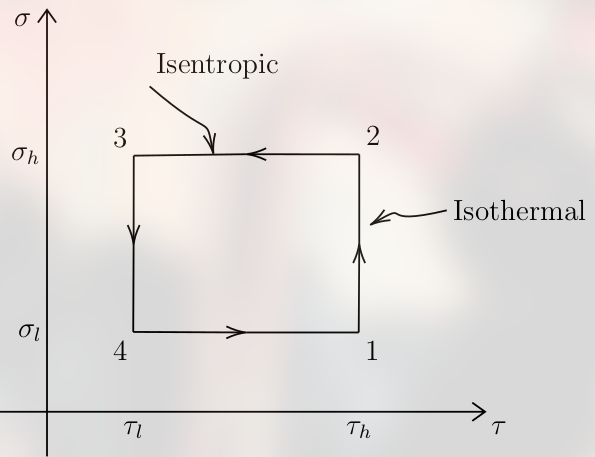
\includegraphics[width=.35\textwidth]{Figures/CCycle.png}

    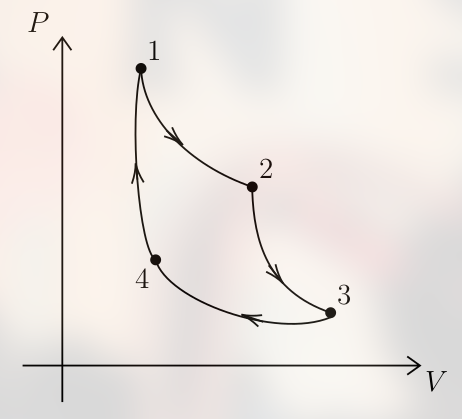
\includegraphics[width=.35\textwidth]{Figures/IdealCCycle.png}

\end{multicols}

\end{document}

